\section{Электростатика}

%1
\AddProb Два маленьких шарика, массы которых $m$ и $M$, заряжены одинаковыми зарядами $q$ и удерживаются на расстоянии $L$ друг от друга. 
Шарики отпускают, и они начинают разлетаться. Найти скорости шариков после разлета на большое расстояние. 
Найти скорости шариков после разлета на расстояние $7L$.

\AddProb Точечный заряд $q$ находится между двумя заземленными проводящими концентрическими сферами 
радиусами $a$ и $b$ на расстоянии $r$ от центра ($a~<~r~<~b$). 
Найти полные индуцированные на сферах заряды. Рассмотреть все возможные предельные случаи.

\begin{wrapfigure}{r}{3cm}
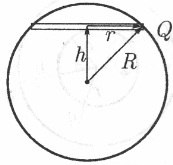
\includegraphics[width=3cm]{1003ElectrostaticsBall.jpg}
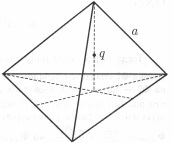
\includegraphics[width=3cm]{1004ElectrostaticsTetrahedron.jpg}
\end{wrapfigure}

\AddProb Заряженный металлический шар радиуса $R$ разрезан на две части по плоскости, отстоящей от центра на расстояние $h$. 
Найти силу, с которой отталкиваются эти части. Исходный заряд шара~$Q$.

\begin{figure}{h}
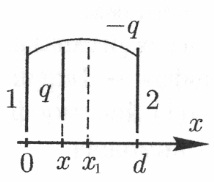
\includegraphics[scale=0.5]{1005ElectrostaticsTwoPlates.jpg}
\end{figure}

\AddProb Грани правильного тетраэдра со стороной $a$ равномерно заряжены с поверхностной плотностью заряда $\sigma$. 
В центр тетраэдра помещен точечный заряд $q$. Найти силу, с которой точечный заряд действует на одну из граней тетраэдра.

\AddProb Две большие проводящие пластины $1$ и $2$ расположены на расстоянии $d$ друг от друга, 
а между ними на расстоянии $х$ от пластины $1$ находится проводящая пластина с зарядом $q$. 
Крайние пластины соединены проводником и имеют заряд $-q$. 
Какой заряд пройдет по проводнику, соединяющему крайние пластины, если пластину с зарядом $q$ переместить из положения $x$ в положение с координатой~$x_1$.

\AddProb (2017) В вакууме относительно некоторой ИСО покоится однородное тонкое кольцо радиуса $R$, массой $3m$ и равномерно распределенным зарядом $q$. Какую минимальную скорость в этой ИСО должна иметь частица массой $m$ и зарядом равным по знаку и величине заряду кольца, чтобы, двигаясь вдоль оси кольца с очень большого расстояния, достичь его центра? Рассмотрите два случая: а) кольцо закреплено; б) кольцо свободное.

\section{Конденсаторы}

\begin{wrapfigure}{r}{4cm}
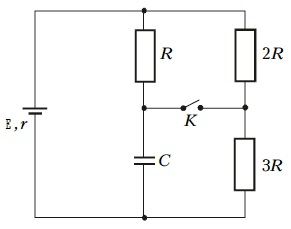
\includegraphics[scale=0.45]{1001Condensers.jpg}
\end{wrapfigure}

%6
\AddProb В электрической схеме, изображенной на рисунке, в начальный момент времени ключ $K$ разомкнут, конденсатор не заряжен. 
Параметры схемы указаны на рисунке. Определите начальные токи через резисторы и через батарею сразу после замыкания.

\begin{wrapfigure}{r}{3.5cm}
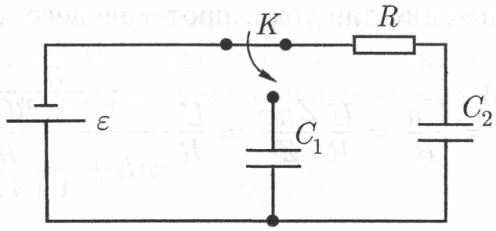
\includegraphics[scale=0.25]{1002Condensers.jpg}
\end{wrapfigure}

\AddProb Батарея с ЭДС, равной {\Large $\varepsilon$}, конденсаторы емкостями $C_1$ и $C_2$ и резистор сопротивлением $R$ соединены так, как показано на рисунке. 
Найдите количество теплоты $Q$, выделяющееся на резисторе после переключения ключа~$K$.

\AddProb По какому закону изменяется ток через конденсатор емкости $C$, подключенный к источнику тока $U$ через сопротивление~$R$?

\AddProb Две батареи включены в схему, изображенную на рисунке (сопротивления всех резисторов равны $R$). 
Первоначально конденсаторы не заряжены, а ключи разомкнуты. Ключи одновременно замыкают. 
1) Найти начальный ток через резистор $R_1$. 2) Какое количество теплоты выделится во всей схеме после замыкания ключей?

\begin{figure}
	\begin{subfigure}{0.5\textwidth}
	\centering
	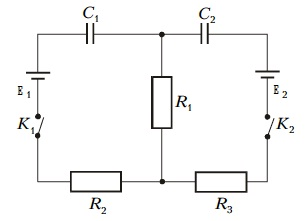
\includegraphics[scale=0.5]{1005Condensers.jpg}
	\end{subfigure}
	\begin{subfigure}{0.5\textwidth}
	\centering
	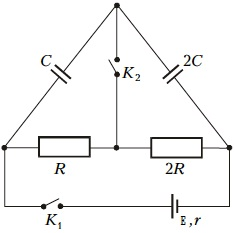
\includegraphics[scale=0.5]{1006Condensers.jpg}
	\end{subfigure}
\end{figure}

\AddProb В схеме на рисунке ключи разомкнуты, а конденсаторы не заряжены. Ключ $K_1$ замыкают, оставляя ключ $K_2$ разомкнутым. 
1) Какие напряжения установятся на конденсаторах? 2) Какой заряд протечет через ключ $K_2$ при замыкании?